





\subsection{Logistic Regression in Perfectly Linearly Separable case}

\begin{figure}[H]
    \centering
    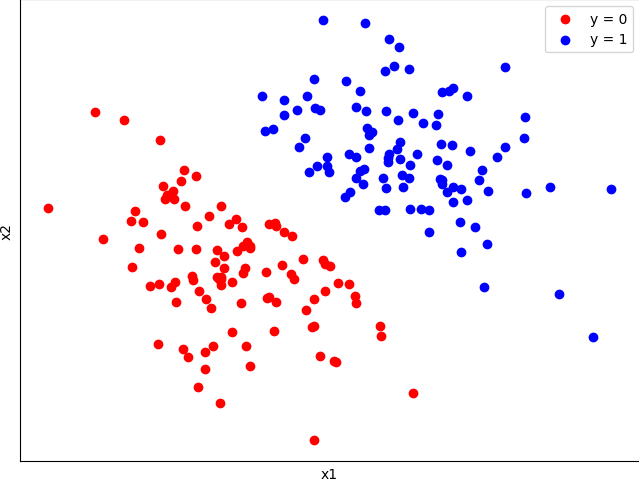
\includegraphics[width=0.5\textwidth]{images/gaussian_separable_data_plot.png}
    \caption{Data for Logistic Regression, features $x_1$ and $x_2$}
    \label{fig:linearly_separable}
\end{figure}

Consider Logistic Regression on \textbf{Perfectly Linearly Separable} data, as shown in \autoref{fig:linearly_separable}. You may not assume that there are just $2$ features as shown in the figure.

\begin{enumerate}[label=\alph*)]
\item What is the condition (possibly implicit) for a data to be linearly separable, when the features $\xieg \in \re^n$.

\item Consider solving for the decision boundary $(\wb, b)$ for such data. Show what $\forall \epsilon > 0 \ \ \exists (\wb_{\epsilon}, b_{\epsilon})$ such that $\loss_{Losgistic}(\wb, b) < \epsilon$.

\item Consider running gradient descent, to obtain $(\wb, b)$. Assuming the learning rate is small, will the algorithm ever converge in $(\wb, b)$? (Answer: $\wb$ and $b$ diverge. You may skip it as it's difficult to prove.)
\end{enumerate}





\subsection{Logistic Regression for multiple classes}

Consider $r$ class classification problem. We build a model that predicted an input belonging to each of the $r$ classes (similar to Logistic Regression).

The model is parametrized by $r$ weight vectors, $\wb_1, \wb_2...\wb_r$. For an input $\xieg$, the model is evaluated as,

\begin{align}
z_j^{(i)} = \wb_j^T \xieg \ \ \text{ for j } = 1,2 ....r\\
\hat{y}^{(i)}_j = \frac{e^{z_j}}{\sum_{k = 1}^{r} e^{z_k}} \ \ \text{ for j } = 1,2 ....r\label{softmax}
\end{align}

\autoref{softmax} is the Softmax function. (Why \textbf{Soft}max?) The loss function, for a single example $(i)$, $\yieg \in \{1,2....r\}$ is
\begin{equation}\label{cross_entropy}
    \loss^{(i)}(\wb_1, \wb_2...\wb_r) = -\sum_{j = 1}^{r} \mathbbm{1}_{\{\yieg = j\}} \log(\yhatieg_j)
\end{equation}

Where $\mathbbm{1}_{(.)}$ is the indicator function.
\[
\mathbbm{1}_{(x)} = 
\begin{cases} 
1 & \text{if } x \text{ is True} \\
0 & \text{if } x \text{ is False}
\end{cases}
\]

\autoref{cross_entropy} is know is the \textbf{Cross Entropy Loss function}. Now, define 
$$\loss(\wb_1, \wb_2...\wb_r) = \sum_{i = 1}^{m} \loss^{(i)}(\wb_1, \wb_2...\wb_r)$$

\begin{enumerate}[label=\alph*)]
\item  Is $\loss(\wb_1, \wb_2...\wb_r)$ convex? (Answer: Yes! But you may skip it as the proof gets very involved.)
\item Obtain explicitly, $\nabla_{\wb_1} \loss, \nabla_{\wb_2} \loss.....\nabla_{\wb_r} \loss$. Hint: Start by writing $\loss$ in terms of $(\wb_1, \wb_2...\wb_r)$.
\end{enumerate}
